%==================================================================================================================================%
%==================================================== 第三章 曲面上的 SCFT 模型 ====================================================%
%==================================================================================================================================%
\chapter{基础多项式空间} \label{Chap:Numerical methods}
重心坐标——参考单元——实体单元之间的关系

\section{重心坐标}
对标准有限元来说, {\bf 重心坐标}是一个非常重要的概念, 它是构造有限元基函数的基础。下面建立重心坐标和笛卡尔坐标之间的关系。

设 $\{\bfx_i = (x_{i,0}, x_{i, 1}, \cdots, x_{i, d-1})^T\}_{i=0}^{d}$ 是 $\mathbb
R^d$ 空间中的 $d+1$ 个点,如果它们不在一个超平面上, 即 $d$ 维向量集合
$\{\bfx_0\bfx_i\}_{i=1}^d$ 是线性独立的,也等价于下面的矩阵非奇异
\begin{equation}
	\bfA =\begin{pmatrix}
		x_{0, 0} & x_{1, 0} & \cdots & x_{d, 0} \\
		x_{0, 1} & x_{1, 1} & \cdots & x_{d, 1} \\
		\vdots   & \vdots   & \ddots & \vdots \\
		x_{0, d-1} & x_{1, d-1} & \cdots & x_{d, d-1}\\
		1 & 1 & \cdots & 1
	\end{pmatrix}
\end{equation}


给定任意点 $\bfx=(x_0, x_1, \cdots, x_{d-1})^T\in \mathbb R^d$, 可以得到一组实数
值 $\lambda := (\lambda_0(\bfx), \lambda_1(\bfx), \cdots, \lambda_d(\bfx))^T$, 满足如下的方程
\begin{equation}
	\bfA \lambda=
	\begin{pmatrix}
		\bfx \\ 1
	\end{pmatrix}
	\label{eq:lbc}
\end{equation}
即
\begin{equation}
	\bfx = \sum\limits_{i=0}^{d}\lambda_i(\bfx) \bfx_i,
	\text{ with} \sum\limits_{i=0}^{d}\lambda_i(\bfx) = 1.
\end{equation}

点集 $\{\bfx_i\}_{i=0}^d$ 的凸壳
\begin{equation}
	\tau = \{\bfx = \sum_{i=0}^{d}\lambda_i\bfx_i | 0\leq \lambda_i \leq
	1, \sum_{i=0}^d\lambda_i = 1\}
\end{equation}
就称为由点集 $\{\bfx_i\}_{i=0}^d$ 生成的几何 $d$-单纯形。 例如, 区间是 1-单纯形,三
角形是一个 2-单纯形, 四面体是一个 3-单纯形。

而 $\lambda_0(\bfx)$, $\lambda_1(\bfx)$, $\cdots$, $\lambda_{d}(\bfx)$ 就称为
$\bfx$
关于点集 $\{\bfx_i\}_{i=0}^d$ 重心坐标。  易知 $\lambda_0(\bfx)$,
$\lambda_1(\bfx)$, $\cdots$, $\lambda_{d}(\bfx)$ 是关于 $\bfx$ 的线性函数并且,
\begin{equation}
	\lambda_i(\bfx_j) = 
	\begin{cases}
		1, & i = j\\
		0, & i\not= j
	\end{cases}, 
	i, j = 0, \cdots, d
\end{equation}

下面我们分别具体写出一维、二维、三维重心坐标与笛卡尔坐标之间的关系,导数表示,及其几何意义。
\subsection{一维重心坐标}
一维重心坐标可由区间端点来表示,给定区间单元$[x_0,x_1]$则对任意的$x \in [x_0,x_1]$,
\begin{figure}[H]
	\centering
	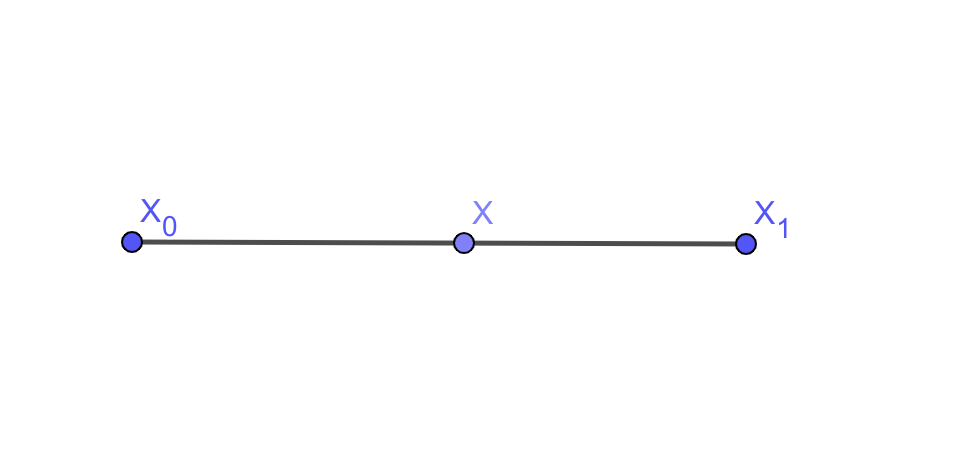
\includegraphics[width=0.7\linewidth]{figures/intervalbc}
	\label{fig:intervalbc}
\end{figure}
定义其上的重心坐标为$(\lambda_0,\lambda_1)$, 满足如下关系
\begin{equation}
	\left[\begin{array}{cc}
		x_{0} & x_{1} \\
		1 & 1
	\end{array}\right]\left[\begin{array}{l}
		\lambda_{0} \\
		\lambda_{1}
	\end{array}\right]=\left[\begin{array}{l}
		x \\
		1
	\end{array}\right]
\end{equation}
因此可以计算出重心坐标的表达式为
\begin{equation}
	\lambda_{0}(x)=\frac{x_{1}-x}{x_{1}-x_{0}}, \lambda_{1}(x)=\frac{x-x_{0}}{x_{1}-x_{0}}
\end{equation}
其关于x的导数为
\begin{equation}
	\frac{d \lambda_{0}}{d x}=\frac{-1}{x_{1}-x_{0}}, \frac{d \lambda_{1}}{d x}=\frac{1}{x_{1}-x_{0}}
\end{equation}

以为重心坐标的几何意义为,对于$[x_),x_1]$上任意一点x的重心坐标$(\lambda_{0},\lambda_{1})$,$\lambda_{0}$表示$x_0$所对的边$[x,x_1]$占整个区间$[x_0,x_1]$长度的比例,$\lambda_{1}$表示$x_1$所对的边$[x_0,x]$占整个区间$[x_0,x_1]$长度的比例


\subsection{二维重心坐标}
二维重心坐标可由三角形三个定点来表示,给定三角形区域$\Omega$,其三个顶点为 ${\bfx_i:x_i=(x_{i0},x_{i1})}i=0,1,2$,
\begin{figure}[H]
	\centering
	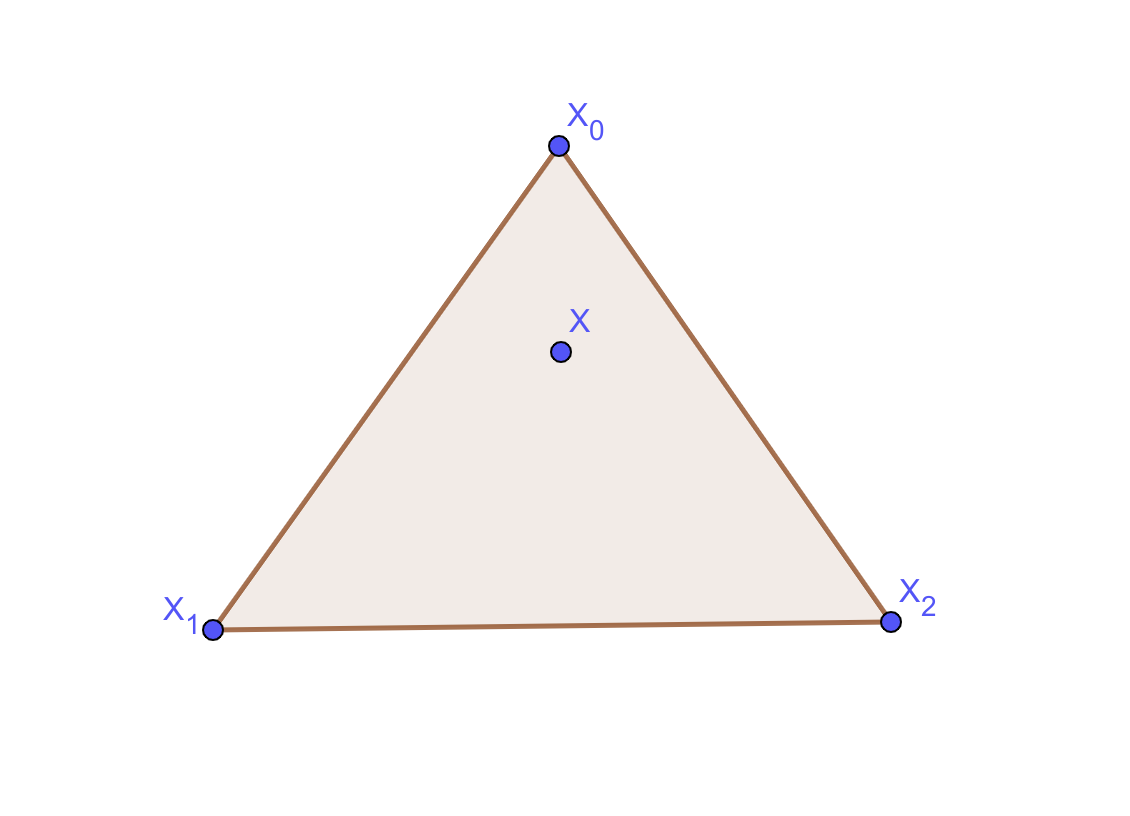
\includegraphics[width=0.7\linewidth]{figures/trianglebc}
	\label{fig:intervalbc}
\end{figure}
则对任意的点$\bfx=(x_0,x_1)\in \Omega$, 定义其上的重心坐标为$(\lambda_0,\lambda_1,\lambda(2))$, 满足如下关系
\begin{equation}
	\left[\begin{array}{ccc}
		x_{00} & x_{10} & x_{20} \\
		x_{01} & x_{11} & x_{21} \\
		1 & 1 & 1
	\end{array}\right]\left[\begin{array}{l}
		\lambda_{0} \\
		\lambda_{1} \\
		\lambda_{2}
	\end{array}\right]=\left[\begin{array}{c}
		x_{0} \\
		x_{1} \\
		1
	\end{array}\right]
\end{equation}
因此可以推出重心坐标的表达式为
\begin{equation}
	\left[\begin{array}{l}
		\lambda_{0} \\
		\lambda_{1} \\
		\lambda_{2}
	\end{array}\right] =
	\left[\begin{array}{ccc}
		x_{00} & x_{10} & x_{20} \\
		x_{01} & x_{11} & x_{21} \\
		1 & 1 & 1
	\end{array}\right]^{-1}
	\left[\begin{array}{c}
		x_{0} \\
		x_{1} \\
		1
	\end{array}\right]
\end{equation}

记
\begin{equation}
	\left[\begin{array}{ccc}
		x_{00} & x_{10} & x_{20} \\
		x_{01} & x_{11} & x_{21} \\
		1 & 1 & 1
	\end{array}\right]^{-1}
	:=
	\left[\begin{array}{lll}
		a_{00} & a_{01} & a_{02} \\
		a_{10} & a_{11} & a_{12} \\
		a_{20} & a_{21} & a_{22}
	\end{array}\right]
\end{equation}

则重心坐标的梯度为

\begin{equation}
	\begin{array}{l}
		\nabla \lambda_{0}=\left[\begin{array}{l}
			\frac{\partial \lambda_{0}}{\partial x_{0}} \\
			\frac{\partial \lambda_{0}}{\partial x_{1}}
		\end{array}\right]=\left[\begin{array}{l}
			a_{00} \\
			a_{01}
		\end{array}\right] \\
		\nabla \lambda_{1}=\left[\begin{array}{l}
			\frac{\partial \lambda_{1}}{\partial x_{0}} \\
			\frac{\partial \lambda_{1}}{\partial x_{1}}
		\end{array}\right]=\left[\begin{array}{l}
			a_{10} \\
			a_{11}
		\end{array}\right] \\
		\nabla \lambda_{2}=\left[\begin{array}{l}
			\frac{\partial \lambda_{2}}{\partial x_{0}} \\
			\frac{\partial \lambda_{2}}{\partial x_{1}}
		\end{array}\right]=\left[\begin{array}{l}
			a_{20} \\
			a_{21}
		\end{array}\right]
	\end{array}
\end{equation}


其几何意义为,对于$\Omega$上任意一点x的重心坐标$(\lambda_{0},\lambda_{1},\lambda_{2})$

\begin{itemize}
	\item $\lambda_{0}$表示$x_0$所对的三角形$\triangle_{x,x_1,x_2}$占整个区间$\triangle_{x_0,x_1,x_2}$面积的比例
	\item $\lambda_{1}$表示$x_1$所对的三角形$\triangle_{x,x_0,x_2}$占整个区间$\triangle_{x_0,x_1,x_2}$面积的比例
	\item $\lambda_{2}$表示$x_2$所对的三角形$\triangle_{x,x_0,x_1}$占整个区间$\triangle_{x_0,x_1,x_2}$面积的比例
\end{itemize}


\subsection{形函数}
\begin{definition}{形函数}
	形函数定义于单元内部的、坐标的连续函数,它满足下列条件:
	\begin{itemize}
		\item 在节点i处,$\lambda_i =1$;在其他节点处,$\lambda_i = 0$;
		\item 能保证用它定义的未知量(u、v或x、y)在相邻单元之间的连续性;
		\item 应包含任意线性项,使用它定义的单元唯一可满足常应变条件;
		\item 应满足下列等式:$\sum \lambda_i(\bfx_i)= 1$。
	\end{itemize}
\end{definition}


\section{拉格朗日空间}
\subsection{区间}
给定一个区间 $[0,1]$, 其所在坐标变量记为 $\xi$ 称这个区间为{\bf 参考区间单
	元}, 简称为{\bf 参考单元}.  易知, 参考单元重心坐标为
\begin{align*}
	\lambda_0 &= 1 - \xi\\
	\lambda_1 &= \xi\\
\end{align*}
给定{\bf 非负多重整数}指标向量 $\bfm_\alpha = (m_0, m_1)$, 在参考单元上可以构造如下的 $p$ 次多项式函数:
\begin{equation}
	\phi_{\alpha} = \frac{1}{\bfm_\alpha!}\prod_{i=0}^{1}\prod_{j_i =
		0}^{m_i - 1} (p\lambda_i - j_i).
	\label{eq:phi}
\end{equation}
其中
\begin{align*}
	&m_0 + m_1 = p,\quad \bfm_\alpha! = m_0!m_1!, \\
	&\prod_{j_i=0}^{-1}(p\lambda_i - j_i) = 1,\quad i = 0, 1.
\end{align*}
$\phi_{\alpha}$ 可以看成 $\xi$ 的函数, 也可以看成 $\lambda
= (\lambda_0, \lambda_1)$ 的函数. 易知, 这样的函数可以定义
$p+1$ 个.
对于每个形函数 $\phi_\alpha$ 对应的 {\bf 非负多重整数}指标向量 $\bfm_\alpha
= (m_0, m_1)$, 都可定义唯一的重心坐标
$$
\lambda_\alpha = (\frac{m_0}{p}, \frac{m_1}{p}).
$$
满足
\begin{equation*}
	\phi_\alpha(\lambda_\alpha) = 1.
\end{equation*}
给定一个不同的{\bf 非负多重整数}指标向量 $\bfm_\beta$, 有
\begin{equation*}
	\phi_\alpha(\lambda_\beta) = 0.
\end{equation*}
\subsection{三角形}
\subsection{四面体}
\section{缩放单项式空间}
\section{Bernstein 多项式}
n次伯恩斯坦多项式定义为
\begin{equation}
	B_{i, n}(t) = \dbinom{n}{i}t^{i}(1-t)^{n-i}
\end{equation}
$i=0,1,\cdots,n,$其中
\begin{equation}
\dbinom{n}{i}t^{i}=\frac{n !}{i !(n-i) !}
\end{equation}
伯恩斯坦多项式也可以通过递归的方法来定义,即
\begin{equation}
	\begin{aligned}
		(1-t) B_{k, n-1}(t)+t B_{k-1, n-1}(t) &=(1-t)\left(\begin{array}{c}
			n-1 \\
			k
		\end{array}\right) t^{k}(1-t)^{n-1-k}+t\left(\begin{array}{c}
			n-1 \\
			k-1
		\end{array}\right) t^{k-1}(1-t)^{n-1-(k-1)} \\
		&=\left(\begin{array}{c}
			n-1 \\
			k
		\end{array}\right) t^{k}(1-t)^{n-k}+\left(\begin{array}{c}
			n-1 \\
			k-1
		\end{array}\right) t^{k}(1-t)^{n-k} \\
		&=\left[\left(\begin{array}{c}
			n-1 \\
			k
		\end{array}\right)+\left(\begin{array}{c}
			n-1 \\
			k-1
		\end{array}\right)\right] t^{k}(1-t)^{n-k} \\
		&=\left(\begin{array}{c}
			n \\
			k
		\end{array}\right) t^{k}(1-t)^{n-k} \\
		&=B_{k, n}(t)
	\end{aligned}
\end{equation}
从定义可以看出,共有n+1个伯恩斯坦多项式。